\documentclass[letterpaper]{article}
\usepackage[utf8]{inputenc}

\usepackage[ngerman]{babel} % Package for translating default language into german e.g. table of contents - Inhaltsverzechnis 


\usepackage{graphicx} % Package for adding pictures
\usepackage{float} % Package for allowing to float images
\graphicspath{ {Pictures/} }

\usepackage{hyperref} % Package for adding urls
\usepackage{fancyhdr} % Package for manipulating header and footer

\usepackage[square, numbers, sort&compress]{natbib} % Package for table of contents
\bibliographystyle{unsrtnat}
\usepackage[nottoc]{tocbibind} % Package for adding References in the table of contents
\usepackage{listings} % Packegs for adding javascript code with code highlighting
\usepackage{xcolor}

\definecolor{lightgray}{rgb}{.94,.94,.94}
\definecolor{Green}{rgb}{0,107,0}
\definecolor{purple}{rgb}{0.65, 0.12, 0.82}

\lstdefinelanguage{JavaScript}{
  keywords={typeof, new, true, false, catch, function, return, null, catch, switch, var, if, in, while, do, else, case, break, class, export, boolean, throw, implements, import, this, constructor, string, number, public, private, static, const, var, let, void},
  keywordstyle=\color{orange}\bfseries,
  identifierstyle=\color{black},
  sensitive=false,
  comment=[l]{//},
  morecomment=[s]{/*}{*/},
  commentstyle=\color{purple}\ttfamily,
  stringstyle=\color{Green}\ttfamily,
  morestring=[b]',
  morestring=[b]"
}

\lstset{
   language=JavaScript,
   backgroundcolor=\color{lightgray},
   extendedchars=true,
   basicstyle=\footnotesize\ttfamily,
   showstringspaces=false,
   showspaces=false,
   tabsize=2,
   breaklines=true,
   showtabs=false,
   captionpos=b
}


\begin{document}

\begin{titlepage}
\begin{minipage}{0.9\linewidth}
\begin{center}
\centering 
	      		 

\includegraphics[width=0.65\linewidth]{hm}
	
\begin{center}
\huge{\textsc{\scshape{ Bachelorarbeit}}}
\end{center}

\vspace{1cm}
{\scshape{\Large Vergleich von Sprachmitteln zur asynchronen Verarbeitung am Beispiel von Typescript\par}}
\vspace{1cm}
    
  
Verfasser  \linebreak
 {\Large Marco Leko\par}
 	\vspace{1.5cm}
angestrebter akademischer Grad\linebreak
 {\Large Bachelor of Science (BSc)\par}
	\vspace{1cm}

\flushleft
\begin{tabular}{ll}
München, 6. Februar 2019\linebreak

\vspace{1cm}&   \\
  Matrikelnummer: & 54442114 \vspace{0.3cm} \\ 
  Studienfach: & Wirtschaftsinformatik \vspace{0.3cm} \\
  Semester: & Wintersemester 2018/2019 \vspace{0.3cm} \\ 
  Betreuer: & Prof. Dr. Bastian Katz \\
 \end{tabular}

\end{center}
\end{minipage}
\end{titlepage}
\setlength{\headheight}{45pt}
\pagestyle{fancy}
\fancyhf{} % clear all header and footer fields
\rhead{
\includegraphics[width=2.8cm,height=1.3cm]{Hochschule_muenchen_logo.jpg}}
\lhead{Hochschule München}
\fancyfoot[C]{\thepage}
\thispagestyle{fancy}
\setcounter{secnumdepth}{0}
\section{Eidesstattliche Erklärung}

Hiermit versichere ich, die vorliegende Bachelorarbeit selbstständig und nur unter Verwendung der von mir angegebenen Quellen und Hilfsmittel verfasst zu haben. Sowohl inhaltlich als auch wörtlich entnommene Inhalte wurden als solche kenntlich gemacht. Die Arbeit hat in dieser oder vergleichbarer Form noch keinem anderem Prüfungsgremium vorgelegen.
\\[1.5cm]
Datum:	\hrulefill\enspace Unterschrift: \hrulefill


\newpage

\section{Danksagungen}
**Meine Danksagung**

\tableofcontents
\setcounter{secnumdepth}{1}

\section{Einführung}

Javascript ist im Aufwind mehr denn je. Sie ist die meist genutzte Programmiersprache unter Entwicklern. Laut der diesjährigen Umfrage von Stackoverflow belegte sie zum sechsten mal in Folge den ersten Platz\cite{programming-language-survey}. Doch woher kommt dieser Erfolg? \\

\noindent
Wenn es um das Web geht, war Javascript als Skriptsprache schon immer Vorreiter. Doch diese Sprache hat seine Stärken auch in der Vielfalt seiner Einsatzmöglichkeiten. Wie mit dem Framework Node.js, dass ab 2009 in Erscheinung getreten ist, war es möglich Server-seitigen Javascript-Code zu implementieren. Dies hatte zur Folge, dass man sich nicht mit multiplen Programmiersprachen auseinandersetzen musste. Man hatte eine Vereinheitlichung in seiner Code-Basis gefunden. Zudem bietet Node.js mit npm als Paketmanager die größte Auswahl an Open-Source-Libraries. Ein weiterer Punkt ist die Multi-Plattform-Kompatibilität die Javascript z.B. mit Angular offenbart. Mit diesem Framework kann man mit einer Code-Basis sowohl Web-Anwendungen als auch Apps für mobile Geräte entwickeln. Diese Hybrid Applikationen werden Progressive Web Apps genannt und können durch optimiertes Caching auch im Offline Modus betrieben werden. Das ist nur möglich, da Javascript's Ausführung vom Betriebssystem unabhängig ist. Und genau das bietet auch Typescript. Da Typescript ein \textit{Superset} von Javascript ist, kann jeder Javascript Code auch in Typescript interpretiert werden. Der Unterschied von Typescript zu Javascript ist die statische Typisierung. Das bedeutet, dass Variablen, Methoden und Funktionsparameter im Vorfeld mit einem Typ versehen werden. Aufgrund dessen können Bugs zur Laufzeit schneller erkannt werden. Zudem lässt sich der Code durch die Kapselung in Objekten leicht modular aufbauen und dokumentieren.\\

\noindent
Doch mit der Vielfalt steigt auch die Komplexität der Sprache. Schon zum vierten Jahr in Folge erschien eine neue Version von Javascript, die neueste Features mit sich bringt. Beispielsweise ermöglichen Promises und async await einen weiteren Ansatz zur asynchronen Verarbeitung. Somit werden Applikation, die ereignisgesteuert operieren, neue Möglichkeiten geboten. Mit Callbacks, Promises und Streams bekommen Entwickler verschiedene Optionen der asynchronen Datenverarbeitung zur Verfügung. Die Einsatzmöglichkeiten in einem Projekt können variieren, jedoch welcher Ansatz in welcher Situation sinnvoller erscheint, ist besonders für Entwickler mit wenig Erfahrung schwer zu erkennen.

\subsection{Zielsetzung}

Ziel der Arbeit ist es die Betrachtung und Aufbereitung des Einsatzes von Sprachmitteln zur asynchronen Verarbeitung in Typescript in einer Form, die Einsteigern in die Thematik hilft, die unterschiedlichen Konzepte voneinander abzugrenzen und richtig einzusetzen. Dazu soll asynchrone Verarbeitung insgesamt anhand brauchbarer und für den Einsatz von Typescript typischer Szenarien motiviert werden. Es werden die zur Verfügung stehenden Sprachmittel wie Callbacks, Promises und Observables mit ihren jeweiligen Features vorgestellt. Nach dem Lesen dieser Arbeit soll der Leser ein gewisses Verständnis dafür gewonnen haben, welche der vorgestellten Sprachmitteln für welchen Anwendungsfall besser geeignet ist.\\

\noindent
Zielgruppe dieser Arbeit sind Personen, die Grundkenntnisse in der Sprache Javascript/Typescript vorweisen können. Des Weiteren sollte man von dem Modell der asynchronen Datenverarbeitung wie Callbacks, Promises und Oberservables schon mal gehört haben, da diese in der Arbeit gegenübergestellt werden.

\subsection{Aufbau}

In dieser Arbeit werden die jeweiligen Ausarbeitungen der Ansätze mit Code-Beispielen unterstützt. Neben simulierten Anwendungsbeispielen zum Einstieg werden auch praxisnahe Beispiele wie z.B. Aufrufe an einer REST-API dargestellt. Das Code-Projekt lässt sich fachlich in den Modulen Callbacks, Promises, Async Await und RxJS unterteilen. Die Module haben jeweils eine introduction.ts Datei zur Einführung, eine stories.ts Datei, die entweder Funktionen oder Klassen anbietet und eine stories-usage.ts Datei, die diese Klassen oder Funktionen ausführt. In den jeweiligen Sektionen wird separat gezeigt, wie die einzelnen Dateien ausgeführt werden. Das Repository für das Projekt ist zu finden unter: 

\begin{center}
\url{https://github.com/MarcoLeko/async-patterns.git}
\end{center}

\noindent
Zu beachten ist, dass vor dem Ausführen des Projektes \textbf{Node.js} auf dem Rechner installiert sein muss, um den integrierten Paket-Manager \textbf{npm} nutzen zu können. Da \textbf{RxJS} nicht von vornherein von Javascript mitgeliefert wird, wird eine sog. \glqq Third-Party Library\grqq{} dafür benötigt. Sobald npm installiert ist, muss in dem Stammverzeichnis des Projekts \textbf{npm install} ausgeführt werden, um die jeweiligen Libraries herunterzuladen. Node.js kann man unter folgendem Link herunterladen:

\begin{center}
\url{https://nodejs.org/en/}
\end{center}

\section{Grundlagen}

\subsection{Typescript}
Typescript. Bereits der Name sagt schon was diese Sprache ausmacht. Sie ist eine typisierte Form der Skriptsprache Javascript. Besonders Javascript-Entwickler sträubten sich Anfangs mit der Sprache auseinanderzusetzen. Die Stärke von Javascript liegt in ihrer Flexibilität und der Tatsache nicht mehr code schreiben zu müssen als man braucht. Doch den Kompromiss den man mit Typescript eingeht, zahlt sich am Ende mit dem Zuwachs der Projektgröße aus. Da der Typescript Kompiler bereits Fehler beim Kompilieren erkennt, stellt sich die Frage, ob man lieber Fehler beim Entwickeln oder in der Produktion eines Projekts entdecken möchte. Dabei ist das \textbf{Tooling} der größte Vorteil von Typescript. Wenn man mit Typ-Annotationen oder mit Libraries, die streng typisiert sind, arbeitet, wird der Code von der Entwicklungsumgebung automatisch dokumentiert. Das heißt beim Entwickeln mit einem Code-Editor wird nicht zusätzlich verlangt, die Dokumentation der benötigten Library zu öffnen, um jeden einzelnen Rückgabetyp der Methode zu sehen. Wenn man nun von einem reinen Javascript-Hintergrund kommt, gibt es so gut wie keine Lernkurve die Sprache zu bewältigen. Das liegt daran, dass jeder valide Code von Javascript auch in Typescript ausführbar ist. Der Lernprozess steigt mit zunehmender Nutzung.

\subsubsection{Beispiel}

\begin{figure}[H]
\begin{lstlisting}[basicstyle=\small]
class Greeter {
    greeting: string;
    constructor (message: string) {
        this.greeting = message;
    }
    greet() {
        return "Hello, " + this.greeting;
    }
}  
\end{lstlisting}
\caption{Typescript Klasse \cite{typescript-example}}
\end{figure}

\begin{figure}[H]
\begin{lstlisting}[basicstyle=\small]
var Greeter = (function () {
    function Greeter(message) {
        this.greeting = message;
    }
    Greeter.prototype.greet = function () {
        return "Hello, " + this.greeting;
    };
    return Greeter;
})(); 
\end{lstlisting}
\caption{Überführung in Javascript \cite{typescript-example}}
\end{figure}

\noindent
Typescript selbst kann nicht selbständig ausgeführt werden. Das heißt in einem Browser oder auf einem Server wird unter Umständen immer noch Javascript genutzt. Mit dem Typescript Compiler werden daher Dateien mit dem Suffix *.ts in *.js überführt. Im oberen Code-Schnipsel wurden die Variablen und die Klassenmethoden nach Typescript-Standard deklariert. Diese Typen werden beim transpilieren in Javascript ignoriert. Der Kompiler prüft dann, ob beim übergeben eines Parameters in den Konstruktor ein String Wert eingesetzt wird. Wenn nicht, wird dies als ein Fehler erkannt. In der vom Kompiler auf Javascript übersetzten Version werden die erstellten Klassen und Typen vollständig eliminiert. Was verbleibt ist die Übersetzung der Methode greet() und des Konstruktors. Zudem werden auch nicht direkt deklarierte (implizite) Typen übersetzt. Wie in diesem Fall wird erkannt, dass die Methode greet() ein Wert vom Typ String zurückgibt. Ungleich wie mit Java oder C\# gewährleistet Typescript aus der streng typisierten Welt rauszufahren.

\begin{figure}[H]
\begin{lstlisting}[basicstyle=\small]
let count: any = 23;

count = 'Oops transformed to string!'
\end{lstlisting}
\caption{Wenn unbekannte Objekte von einem API-Aufruf verarbeitet werden, können diese als any deklariert werden.}
\end{figure}

\noindent
Der Kompiler würde hierbei keinen Fehler anzeigen. Obwohl im Idealfall auf die \textbf{any} Notation verzichtet werden sollte, wird dennoch Javascripts Flexibilität geboten. 

\subsubsection{Kompiler}
Ein großer Vorteil von Typescript ist die Möglichkeit auf verschiedene Javascript/Ecmascript Version zu transpilieren. Wenn bestimmte Browser Javascripts neueste Feature noch nicht unterstützen, kann das Kompilat auf ältere Ecmascript Versionen übersetzt werden. Diese Konfiguration wird mit Hilfe einer \textbf{tsconfig.json} Datei bewältigt. Die Auflistung einer solchen Datei zeigt, dass es sich um das Stammverzeichnis des Projekts handelt. Hier können die Kompiler-Optionen für Typescript gesetzt werden oder Dateien von der Übersetzung ein- oder ausgeschlossen werden. Ein Beispiel für die Konfiguration einer solchen Datei könnte wie folgt aussehen: 

\begin{figure}[H]
\begin{lstlisting}[basicstyle=\small]
{
  "compilerOptions": {
    "target": "esnext",
    "module": "commonjs",
    "lib": ["dom", "es2018"],
    "typeRoots": [
      "node_modules/@types"
    ]
  }
}
\end{lstlisting}
\caption{Auflistung einer tsconfig.json Datei}
\end{figure}

\noindent
Mit dem Wert “target” wird die ausgeführte Javascript Version eingestellt. Wenn der Wert nicht bestimmt ist, wird standardmäßig nach es3 übersetzt. Um stets die aktuellste Version zu nutzen, wird für das Projekt \textbf{esnext} angegeben. Typescript wird im Terminal unter dem Verzeichnis einer Typescript-Datei mit \textit{tsc Dateiname.ts} kompiliert. In den für diese Arbeit genutzten Code-Beispielen werden die Startskripte von npm ausgeführt.

\begin{figure}[H]
\begin{lstlisting}[basicstyle=\small]
  ...
  "scripts": {
    "start": "webpack --watch",
    "build": "webpack"
  },
  ...
\end{lstlisting}
\caption{Auflistung ist unter der \textbf{package.json} Datei zu finden}
\label{npm-ex-script}
\end{figure}

\noindent
Wie man in Abbildung \ref{npm-ex-script} sehen kann, führt \textbf{npm run start} nicht tsc aus, sondern \textbf{webpack --watch} aus. Webpack ist ein sog. \textbf{Module-Bundler}. Das Projekt ist nicht nur fachlich, sondern auch technisch in Modulen gegliedert. Diese Module sollten nach Möglichkeit einzeln ausgeführt werden. Ein Module-Bundler läuft während des Build-Prozesses und erfüllt im Wesentlichen zwei Aufgaben. Den Code mit dem Typescript-Kompiler in Javascript zu transpilieren und die daraus resultierenden Kompilate in einer zentralen Datei (main.js) zu bündeln. Um das zu erreichen, nimmt Webpack eine Eingangsdatei als Einstiegspunkt an und bündelt den Inhalt inklusive aller involvierten Importe. Welchen Mehrwert hat Webpack also für das Projekt? \\

\noindent
Beim Ausführen der Beispiele muss nicht jedes mal die jeweilige TS-Datei in eine JS-Datei überführt und das erstellte Kompilat daraufhin in die HTML-Datei referenziert werden. Die HTML-Datei hat nur das Bündel main.js als Referenz und je nach definiertem Einstiegspunkt in der \textbf{webpack.config.js} wird ein neues Bündel erzeugt. Mit der Einstellung \textbf{--watch} werden Veränderung des Codes in Echtzeit kompiliert. Sollten nun Änderungen im Code vorgenommen werden, erstellt Webpack ein neues Bündel. Nach dem Kompilieren muss nur noch die HTML-Seite geöffnet/aktualisiert werden. Um mehr von Typescript und dessen Nutzung mit Webpack zu erfahren, findet unter folgendem Link mehr dazu:

\begin{center}
\url{https://webpack.js.org/guides/typescript/} 
\end{center}

\subsection{Terminologie}

Um die Abgrenzung von verschiedenen asynchronen Sprachmitteln zu beherrschen, muss vorerst geklärt werden, was Asynchronität bedeutet.\\

\noindent
Der zentrale Teil eines Computers, welches Programme und einzelne Schritte zum Ausführen bringt, ist der Prozessor. Die Geschwindigkeit in der eine Schleife von einem Programm ausgeführt wird, hängt von der Geschwindigkeit des Prozessors ab. Programme interagieren jedoch mit Operationen außerhalb des Zuständigkeitsbereiches eines Prozessors, wie z.B. die Kommunikation über ein Netzwerk oder das Abfragen von Daten von der Festplatte. Solche Operationen hängen von anderen Ressourcen ab und brauchen Zeit. In solchen Szenarien wäre es unvorteilhaft, wenn der Prozessor, anstatt andere Operationen in der Zwischenzeit auszuführen, im Leerlauf stecken würde. Genau für solche Aufgaben ist das Betriebssystem da. Das Betriebssystem sorgt dafür, dass Kapazitäten des Prozessors auf parallel laufende Programme wechselt, während es auf die Antwort von ausgeführten Operationen wartet. Es entstehen dabei verschiedene \glqq Threads\grqq{}. Und hier kommt die Asynchronität ins Spiel:

\subsubsection{Asynchronität}

Ein \textbf{asynchrones} Programmiermodell erlaubt multiple Abläufe zum selben Zeitpunkt. Wenn eine Aktion ausgeführt wird, läuft das Programm in einem anderen \glqq Thread\grqq{} weiter. Sollte die Operation fertig gestellt sein, wird das Programm informiert und liefert das Ergebnis zurück. Ein Beispiel dafür wäre das Suchen von Dateien auf einer Festplatte\cite{asynchronitaet}.

\subsubsection{Synchronität}

In einem \textbf{synchronen} Programmiermodell entstehen Abläufe sequenziell. Wenn eine Funktion mit einer zeitintensiven Aktion abgerufen wird, wird das Ergebnis erst nach dem Beenden der Operation zurückgegeben. In diesem Zeitintervall werden keine Nebenoperationen ausgeführt\cite{asynchronitaet}.\\

\noindent
Man kann ein synchrones und asynchrones Modell mit einem kleinem Beispiel vergleichen: Eine Anwendung die zwei Ressourcen aus einem Netzwerk anfragt und die Ergebnisse miteinander kombiniert. In einer synchronen Umgebung würde man dies mit einem Funktionsaufruf nach dem anderen bewältigen. Das hat den Nachteil, dass die zweite Funktion erst dann ausführt, wenn die erste fertig ist. Die Gesamtzeit der Ausführung ist die Summe der Antwortzeiten der beiden Anfragen. Die Lösung dafür ist ein synchrones Programmverhalten mit mehreren kontrollierten Threads. Ein Thread ist ein Ausführungsstrang, der seine eigene Zeitleiste besitzt und innerhalb dieser Operationen ausführt. Ein zweiter Thread könnte zum selben Zeitpunkt die Funktion aufrufen und wenn beide Threads das Ergebnis geliefert bekommen resynchronisieren sie sich und kombinieren ihre Ergebnisse\cite{asynchronitaet}. Im folgenden Diagramm wird ein synchrones Modell mit einem Thread, mit zwei Threads und ein asynchrones Modell gegenübergestellt.

\begin{center}
\begin{figure}[H]
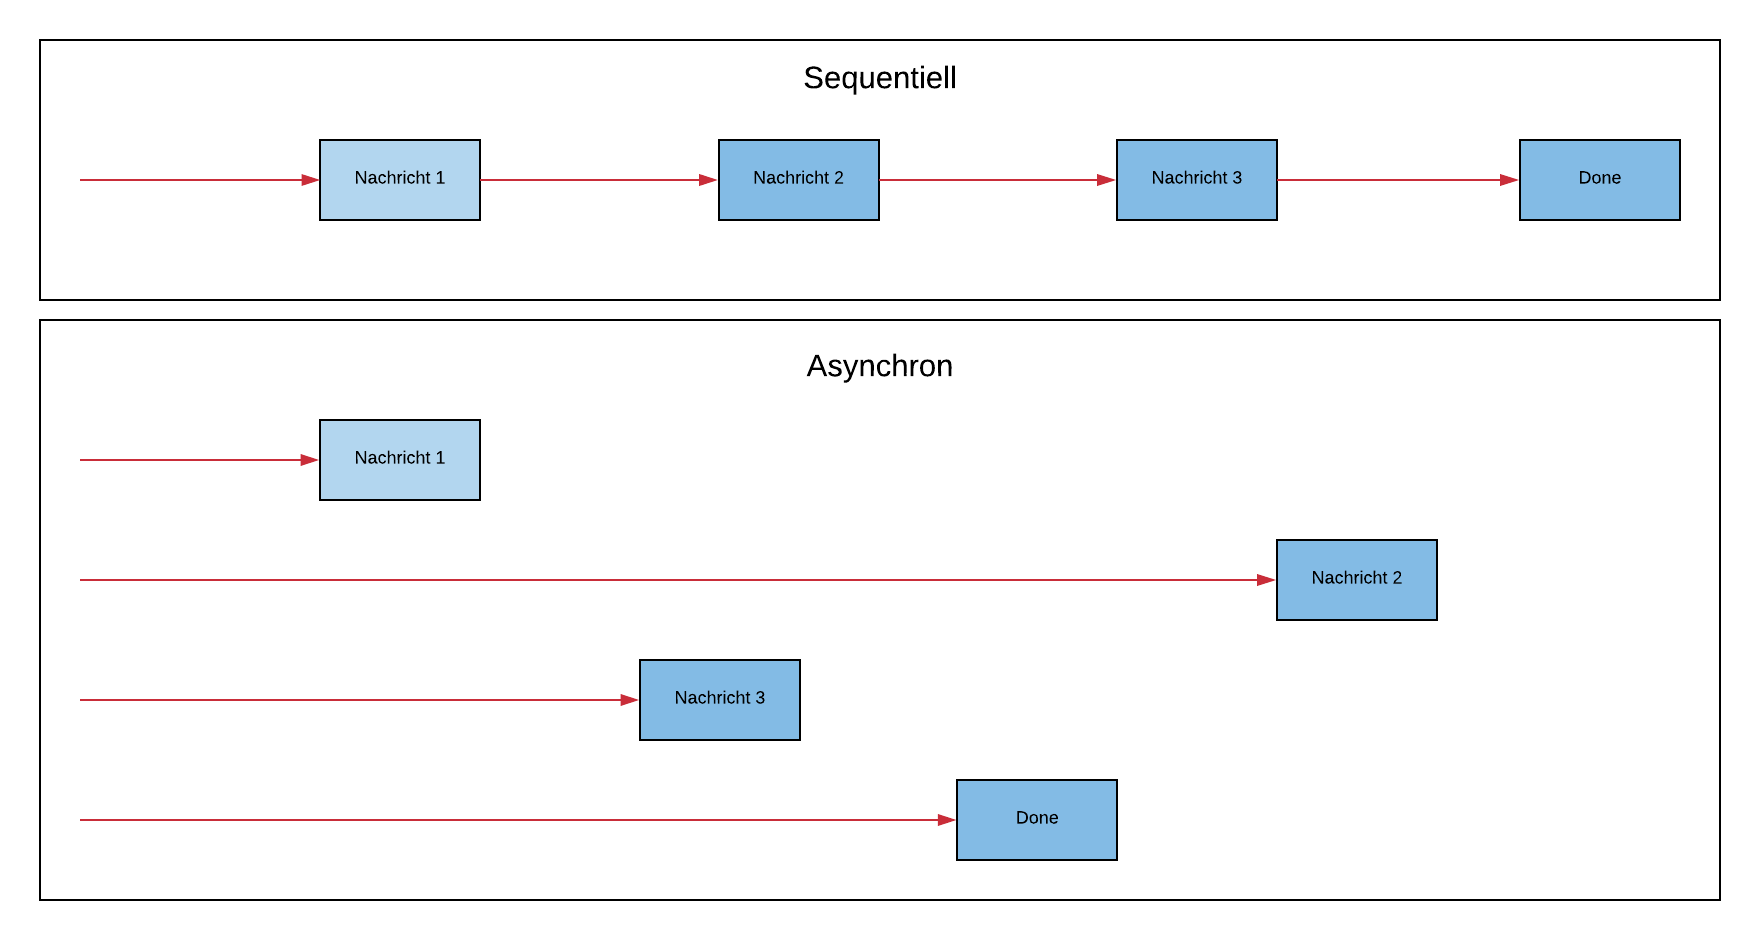
\includegraphics[width=12cm]{synchron-vs-asynchron-diagram}
\caption{Die blauen Linien repräsentieren die Zeit, in der das Programm ausführt und die roten Linien repräsentieren die Zeit, in der auf die Antwort gewartet wird.}
\end{figure}
\end{center}

\noindent
Im synchronen Modell ist die Zeit der Netzwerkanfrage ein Teil der Zeitleiste. Im asynchronen Modell hingegen führt das Starten einer asynchronen Operation zu einer neuen Zeitleiste. Zusammenfassend kann man also sagen, dass in dem synchronen Modell implizit auf die Aktionen gewartet wird, und in dem Asynchronen explizit.
\section{Promises}

Das Prinzip der asynchronen Verarbeitung, bringt Komplexität nach sich. Um dem entgegenzuwirken, hat man in dieser Arbeit schon das Prinzip der Callbacks kennengelernt. Dank der Rückruffunktionen ist es Möglich auf blockierende Aktionen zu warten bis diese eingetroffen sind. Sollten jedoch mehrere asynchrone Events voneinander Abhängig sein, kann das schnell zu unübersichtlichem Code führen (siehe Abb. 6). Mit Promises können voneinander abhängige Events übersichtlich dargestellt werden.\\

\noindent
Ein Promise repräsentiert ein Objekt das noch nicht absehbar ist, aber in Zukunft genutzt werden soll. Als Beispiel könnte man den Inhalt einer Datei, die von einem File-Server in einem Browser geladen werden soll, nehmen. Dieser ist auf Anhieb nicht verfügbar, da die Daten zunächst über das Netzwerk übertragen werden müssen. Anstatt auf den Download zu warten, führt der Browser diesen Prozess asynchron aus. Wenn die Daten angekommen sind, führt das Promise-Objekt die Aktionen mit den erstellten Verarbeitungsmethoden fort. Dank der Promise-Verkettung ist es auch möglich Fehlerbehandlungen übersichtlich abzudecken. Während bei Callbacks das Ergebnis der Interaktion sofort verarbeitet werden muss, basieren Promises nach ihrem Verarbeitungsstatus. Das heißt sie können mit dem Ergebnis auch \glqq{}später\grqq{} interagieren.

\subsection{Funktionsweise}

\noindent
Promises \textit{(zu deutsch: Versprechen)} verhalten sich in Javascript ähnlich wie im echten Leben. Die Definition aus dem Wörterbuch ist: Das Versprechen ist eine einseitige Zusage über eine zukünftige Handlung oder ein zukünftiges Ereignis. \cite{versprechen} \\

\noindent
Das heißt:

\begin{enumerate}
    \item Ein Versprechen ist eine Absicherung, dass etwas gemacht wird. Unabhängig davon, ob das Versprechen sich selbst oder von einer anderen Partei gegeben wird.
    
    \item Ein Versprechen kann eingehalten oder gebrochen werden.
    
    \item Wurde ein Versprechen nicht eingehalten, möchte man den Grund für die Nichteinhaltung wissen, um darauffolgend zu handeln.
    
    \item Beim Zeitpunkt eines Versprechens hat man nur die Absicherung. Man kann damit erstmal noch nichts anfangen. Es kann nur geplant werden was nach dem Einhalten des Versprechens gemacht wird. Dementsprechend kann man auch Maßnahmen setzen beim Nichteinhalten dieser Absicherung.
    
\end{enumerate}

\noindent
Dabei gibt es zwei grundlegende Prinzipien der Promises, die zu Verstehen sind: Das \textbf{Erstellen von Promises} und das \textbf{Verarbeiten von Promises}.

\subsubsection{Erstellen eines Promises}

\begin{figure}[H]
\begin{lstlisting}[basicstyle=\small]
new Promise( /* executor */ (resolve, reject) => { ... } );
\end{lstlisting}
\caption{Erzeugung einer neuen Promise-Instanz}
\end{figure}

Der Konstruktor nimmt eine Rückruffunktion als Eingangsparameter. Diese Funktion wird auch \textbf{Executor} genannt.\cite{promise-executor} Der Executor akzeptiert zwei Parameter \textbf{resolve} und \textbf{reject}. Innerhalb dieser Funktion wird eine asynchrone Operation initiiert (z.B. Das suchen einer Datei, eine Datenbankabfrage etc.). Wurde diese asynchrone Operation erfolgreich ausgeführt, ruft der Promise-Konstruktor die resolve Funktion mit dem entsprechendem Ergebnis auf. Anders wird bei einem Fehler die reject Funktion mit der jeweiligen Fehlernachricht aufgerufen. Zur Einführung ein einfaches Beispiel:\\

\noindent
Vor dem Ausführen des Beispiels sollte ../promises/introduction.ts als Eingangsdatei in der webpack.config.js definiert werden.

\begin{figure}[H]
\begin{lstlisting}[basicstyle=\small]
const keepsHisWord = true;
const resolveRightAway = new Promise((resolve, reject) => {
    if (keepsHisWord) {
        resolve('Promises kept!');
    } else {
        reject('Promise NOT kept!');
    }
});

console.log(resolveRightAway);
\end{lstlisting}
\end{figure}

\noindent
Promises haben einen Status und einen Wert. Bei der Initialisierung einer Promise-Instanz ist der Status erstmals immer ausstehend. In diesem Beispiel löst sich das Promise auf Anhieb vom ausstehenden in den eingetroffenen (resolved) Zustand auf, da die abhängige boolean-Variable vorher auf true gesetzt wurde. Umgekehrt, würde die boolean Variable auf false gesetzt werden, würde der Status abgelehnt (rejected) entsprechen.

\begin{figure}[H]
\centering
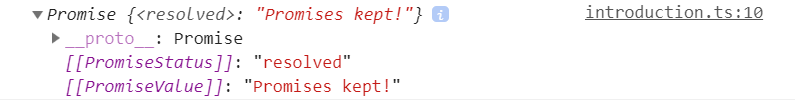
\includegraphics[width=12cm]{promise-beispiel-1}
\caption{}
\end{figure}

\noindent
Der Initialstatus eines Promise wird im nächsten Beispiel verdeutlicht:

\begin{figure}[H]
\begin{lstlisting}[basicstyle=\small]
export interface FakeHttpResponse {
    code: string;
    message: string;
}

const pendingPromise = new Promise<FakeHttpResponse>((resolve, reject) => {
    setTimeout(() => {
        resolve({
            code: '200',
            message: 'Promise kept!'
        });
    }, 10 * 1000);
});

console.log(pendingPromise);
setTimeout(() => console.log(pendingPromise), 10 * 1000);
\end{lstlisting}
\end{figure}

\noindent
Im oberen Beispiel wird das Promise vorbehaltlos nach zehn Sekunden aufgelöst, solange ist der Status ausstehend (pending). Nachdem das Promise aufgelöst wurde, werden Status und Wert aktualisiert. Dabei können nicht nur primitive Typen wie number, boolean oder strings zurückgegeben werden, sondern auch Objekt-Typen und komplexe Typen. Mit anderen Worten: Promises sind generisch.

\begin{figure}[H]
\centering
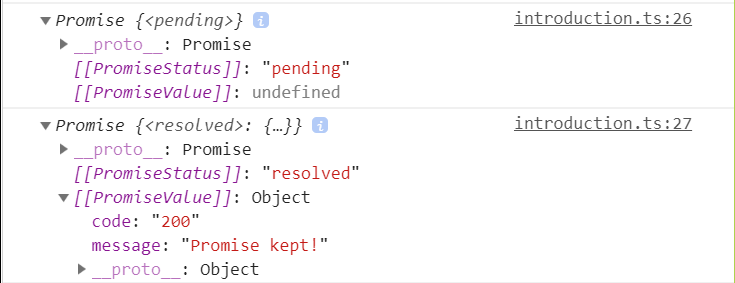
\includegraphics[width=12cm]{promise-beispiel-2}
\caption{Promise hat anfangs den Status \glqq{}ausstehend\grqq{}}
\end{figure}

\noindent
Wie man nun gesehen hat kann ein Promise Objekt den Status \textbf{pending}, \textbf{resolved} oder \textbf{rejected} haben. Im Status pending ist der Ausgang der Aktion noch ungewiss und deshalb der Promise-Wert undefined. Ändert sich der Status bzw. ist die Aktion zum Promise eingetroffen oder fehlgeschlagen, ist der Status \textbf{settled}. Grundsätzlich läuft ein Promise also vom pending in den settled Status. In der nächsten Sektion wird auf das Verarbeiten von Promises näher eingegangen.

\subsubsection{Verarbeiten von Promises}

Zur Wiederholung: Ein Promise-Objekt repräsentiert das eventuelle Eintreffen oder Fehlschlagen einer asynchronen Operation, einschließlich des entstandenen Wertes. Ein solches Objekt bietet \textbf{statische}- und \textbf{Prototyp}-Methoden. Die statischen Methoden können unabhängig von der Instanz aufgerufen werden, während die Prototyp-Methoden nur mit einer Promise Instanz aufrufbar sind. Eine oder mehrere der drei Prototyp-Methoden werden aufgerufen, wenn ein Promise in den settled Zustand eingetroffen ist:

\begin{description}

\begin{figure}[H]
\item \begin{lstlisting}[basicstyle=\small]
Promise.prototype.then(onFulfilled, onRejected)
\end{lstlisting}
\end{figure}

\begin{figure}[H]
\item \begin{lstlisting}[basicstyle=\small]
Promise.prototype.catch(onRejected)
\end{lstlisting}
\end{figure}
 
\begin{figure}[H]
\item \begin{lstlisting}[basicstyle=\small]
Promise.prototype.finally(onFinally)
\end{lstlisting}
\end{figure}
 
\end{description}


\noindent
Die untenstehende Grafik zeigt den Ablauf für das Eintreten der Events (onFulfilled, onRejected und onFinally) und wie man diese verarbeitet. Mit den Methoden \textbf{then()} und \textbf{catch()} werden auf eintretenden Aktionen reagiert. Diese Verarbeitungsmethoden werden aufgerufen wenn ein Promise in den settled Zustand angekommen ist. Im Erfolgsfall wird das Promise mit der then() Methode weiterverarbeitet. Im Fehlerfall hingegen wird die catch() Methode aufgerufen. Da beide Methoden ein Promise-Objekt zurückgeben, können Promises reibungslos aneinandergekettet werden. Wenn \textbf{finally()} an ein Promise Objekt angebunden wird, wird diese Methode in jedem Fall aufgerufen, unabhängig davon ob das Promise eingetroffen oder fehlgeschlagen ist.


\begin{figure}[H]
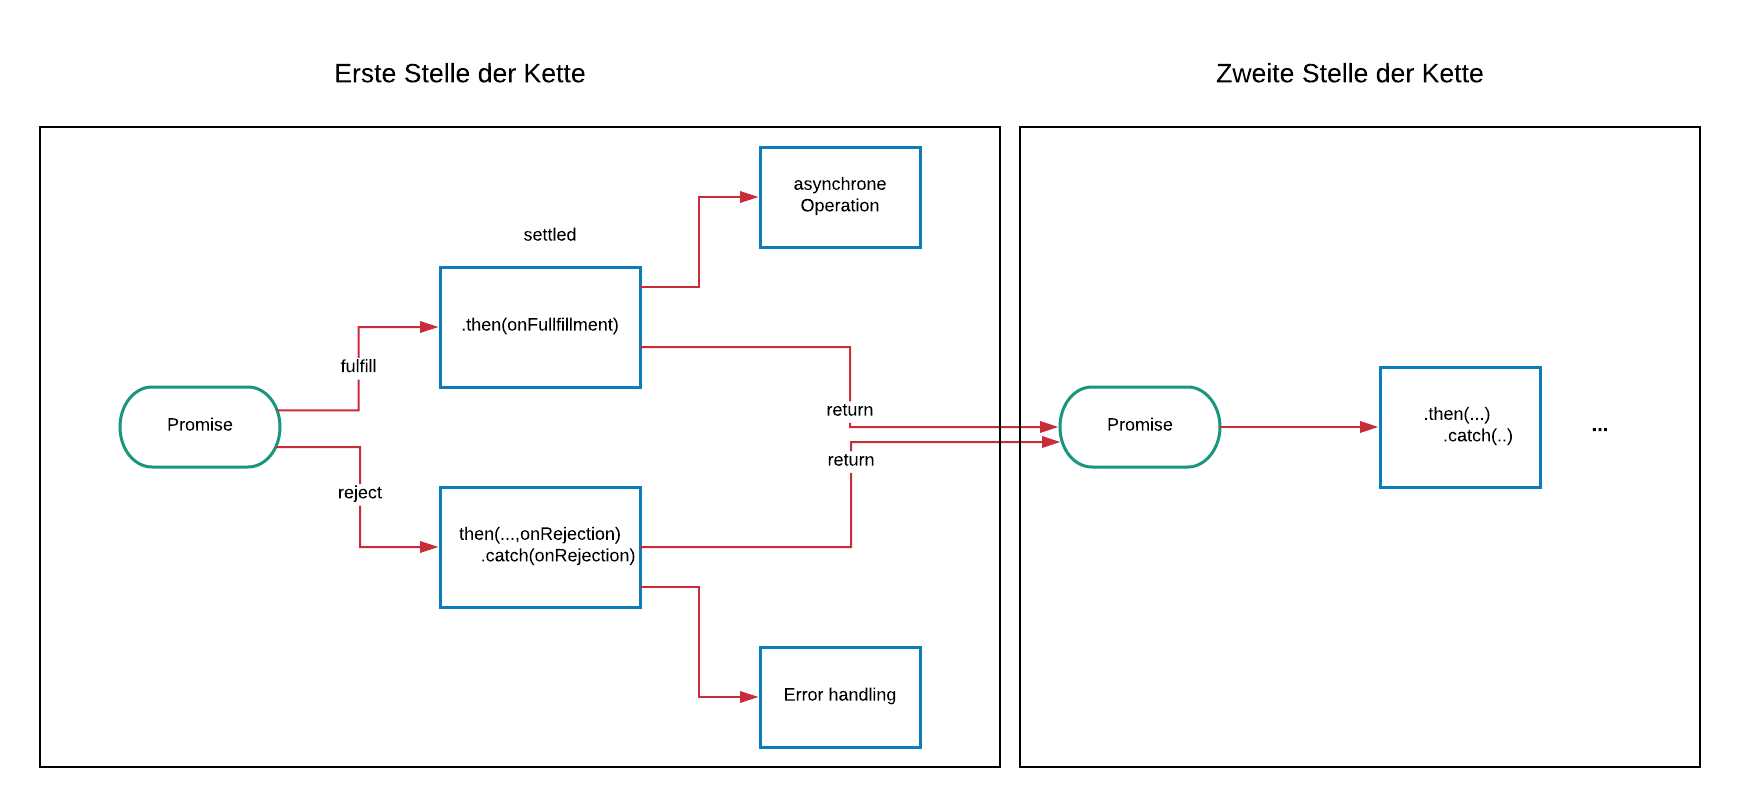
\includegraphics[width=13cm]{Promises-workflow}
\caption{Weiterreichung eines Promise-Objekts \cite{promise-executor}}
\end{figure}

\noindent
Promise-Fehlschläge können dabei auf zwei verschiedene Wege gefangen werden. Innerhalb der then()-Methode kann eine zweite, optionale Funktion für das \textbf{Nicht-Eintreffen} der Operation festgelegt werden. Ein Beispiel dafür wäre:

\begin{figure}[H]
\begin{lstlisting}[basicstyle=\small]
get('story.json').then((response) => {
  console.log('Success!', response);
}, (error) => {
  console.log('Failed!', error);
})
\end{lstlisting}
\caption{Error-Handling innerhalb der then()-Methode. \cite{callback-vs-promises}}
\end{figure}

\begin{figure}[H]
\begin{lstlisting}[basicstyle=\small]
get('story.json').then((response) => {
  console.log('Success!', response);
}).catch((error) => {
  console.log('Failed!', error);
})
\end{lstlisting}
\caption{Error-Handling mit der catch()-Methode. \cite{callback-vs-promises}}
\end{figure}

\noindent
Im Gegensatz zur oberen Variante führt die catch()-Methode keine zusätzlichen Operationen aus. Sie macht den Code lediglich semantisch lesbarer. Wichtig zu beachten ist, dass innerhalb einer Executor-Funktion \textbf{niemals} beide Argumente gemeinsam eintreffen können. Sie verhalten sich exklusiv. Deshalb ist das letztere Beispiel im Verhalten vergleichbar mit diesem Beispiel:

\begin{figure}[H]
\begin{lstlisting}[basicstyle=\small]
get('story.json').then((response) => {
  console.log('Success!', response);
}).then(undefined, (error) => {
  console.log('Failed!', error);
})
\end{lstlisting}
\end{figure}

\noindent
Der Unterschied ist minimal, aber extrem hilfreich. Promise-Fehlschläge gelangen bei der nächsten then()-Methode in den fehlgeschlagen Callback weiter oder in die catch Methode(,wenn vorhanden). Mit then(func1, func2) wird entweder die erste oder die zweite Funktion aufgerufen, aber niemals beide. Jedoch mit then(func1).catch(func2) werden beide Callbacks aufgerufen, sollte die erste Funktion fehlschlagen. Dies ist nur Möglich, da die Funktionen in unterschiedlichen Stellen der Verkettung liegen. Neben den Prototyp-Methoden gibt es, wie bereits erwähnt, die statischen Methoden. Diese bestehen aus vier Methoden:

\begin{itemize}
\item Promise.resolve()
\item Promise.reject()
\item Promise.race()
\item Promise.all()
\end{itemize}

\noindent
Die ersten beiden Methoden werden genutzt um einen eingetroffenen oder fehlgeschlagenen Promises zu simulieren:

\begin{figure}[H]
\begin{lstlisting}[basicstyle=\small]
const rejectedPromise = Promise.reject('I reject on purpose');

rejectedPromise.catch((err: string) => {
    console.log('Reason of failure: ' + err);
});
\end{lstlisting}
\end{figure}

\noindent
Diese Methoden können sich bei der Fehlersuche oder beim Testing als nützlich erweisen. Die anderen beiden Methoden helfen Promises leichter zu verarbeiten. Beispielsweise, wenn es darum geht mehrere Promises auszuführen, hat man entweder die Wahl die Promise-Verkettung zu nutzen oder die Promises in einem Array zu lagern und dann die nötigen Aktionen mit der Sammlung von Promises auszuführen. Im nächsten Beispiel wird die \textbf{Promise-Verkettung}, \textbf{Promise.all()} und \textbf{Promise.race()} gegenübergestellt. Zum Ausführen des Beispiels muss ../promises/stories.ts als Eingangsdatei konfiguriert werden.


\begin{figure}[H]
\begin{lstlisting}[basicstyle=\small]
export class HTTP {

    public makeRequest(url: string): Promise<any> {
        return new Promise((resolve, reject) => {
            const req = new XMLHttpRequest();
            req.open('GET', url);

            req.onload = () => {
                if (req.status === 200) {
                    this.fakeLatency()
                        .then(() => resolve(JSON.parse(req.response)));
                } else {
                    reject(Error(req.statusText));
                }
            };

            req.onerror = () => {
                reject(Error('Network Error'));
            };

            req.send();
        });
    }

    private fakeLatency() {
        return new Promise((resolve) =>
            setTimeout(resolve, 3000 * Math.random()));
    }
}
\end{lstlisting}
\end{figure}

\begin{figure}[H]
\begin{lstlisting}[basicstyle=\small]
export class Story {

    public static BASE_URL = 'https://jsonplaceholder.typicode.com/posts/';
    public spinnerElement: HTMLElement;

    public http: HTTP = new HTTP();

    constructor() {
       this.spinnerElement = Story.createElm('<svg>..</svg>');
    }

    public static createElm(innerHTML: string): HTMLElement {
        const div = document.createElement('div');
        div.innerHTML = innerHTML;
        document.body.appendChild(div);
        return div;
    }
    
    public getAllStories(): Promise<string> {
        return this.http.makeRequest(Story.BASE_URL);
    }

    public getChapter(chapter: number): Promise<string> {
        return this.http.makeRequest(Story.BASE_URL + chapter.toString());
    }
\end{lstlisting}
\end{figure}

\begin{figure}[H]
\begin{lstlisting}[basicstyle=\small]
    public spawn(content): void {
        if (content instanceof Array === false) {
            content = [content];
        }

        content.forEach(elm => {
            const snippet = document.createElement('div');
            snippet.innerHTML = '<h1>${elm.title}</h1>
                                 <div>
                                     <i>${elm.id}</i>
                                 </div>
                                 <p>${elm.body}.</p>';

            document.body.insertBefore(snippet, this.spinnerElement);
        });

    }

    public displayFinished(): void {
        this.spinnerElement.style.display = 'none';
        Story.createElement('All done!');
    }
}

const story = new Story();
\end{lstlisting}
\end{figure}

\noindent
Ähnlich wie im Beispiel des Callback-Kapitels wird von der REST-Api JSONPlaceholder Kapitel in die DOM geladen. In diesem Fall wurde hingegen das objektorientierte Paradigma gewählt. Die Klasse \textbf{HTTP} stellt mit makeRequest() eine Methode zur Verfügung, die eine Http-Anfrage gegen einen übergebenen Endpunkt macht. Mit der \textbf{Story} Klasse wird der Endpunkt der Datenabfrage als Klassenvariable definiert. Darüberhinaus werden mit getAllStories() und getChapter() die Methoden für die Abfrage definiert. Sollte ein Anwendungsfall sein, alle Kapitel anzuzeigen, würde der Code mit Promises so aussehen:

\begin{figure}[H]
\begin{lstlisting}[basicstyle=\small]
story.getAllStories()
    .then((response: XMLHttpRequestResponseType) =>
        story.spawn(response)
    )
    .finally(() =>
        story.displayFinished()
    );
\end{lstlisting}
\end{figure}

\noindent
Alle Kapitel werden mit einem Aufruf am Endpunkt angefragt. Ist das Promise in den settled Zustand angelangt, werden die Kapitel im Browser abgebildet. Als letzte Stelle der Kette wird mit finally der Lade-Icon ausgeblendet und eine Nachricht angezeigt, dass alle Stories abgebildet wurden. Sollte jedoch ein Anwendungsfall sein, dass nur drei Stories im Browser angezeigt werden sollen, könnte das wie folgt aussehen: 

\begin{figure}[H]
\begin{lstlisting}[basicstyle=\small]
story.getChapter(1).then(response1 => // (*)
    story.spawn(response1)
).then(() => // (**)
    story.getChapter(2).then(response2 => story.spawn(response2))
).then(() => // (***)
    story.getChapter(3).then(response3 => story.spawn(response3))
).finally(() =>  // (****)
    story.displayFinished()
);
\end{lstlisting}
\caption{Promise-Verkettung für sequentielle Ausführungen}
\end{figure}

\noindent
In diesem Fall werden nacheinander drei Kapitel angefragt und im Browser angezeigt. Da die Aufrufe im verketteten Konstrukt voneinander abhängig sind, addiert sich die Zeit die gebraucht wird, um ein Kapitel anzufragen und abzubilden. Die Idee dahinter ist, dass nach jedem Kapitelaufruf und -anzeige gewartet wird, bis dieser Vorgang abgeschlossen ist. Der Fluss sieht dabei so aus:

\begin{enumerate}
    \item Das initiale Promise wird aufgerufen und das Kapitel angezeigt. Das Promise gelangt in den settled Status. (*)
    \item Die nächste Stelle der Sequenz wird gestartet, diese endet erst, wenn die Operation innerhalb der then() Methode erfüllt ist (**)
    \item Die nächste Stelle der Sequenz wird initiiert...(***)
\end{enumerate}

\begin{figure}[H]
\centering
\includegraphics[width=12cm]{Promise-Verkettung-Stories.png}
\end{figure}

\noindent
Dieser Vorgang endet mit der finally() Verarbeitungsmethode. Zu beachten ist, dass das gesamte Verkettete Konstrukt in einem eigenen Thread läuft. Innerhalb dieses Threads verlaufen die Operationen jedoch sequentiell. Selbst bei einer weiteren Verzögerung der Kapitel innerhalb der Kette, wäre immer noch gewährleistet, dass die Kapitelaufrufe sequentiell ausgeführt werden:

\begin{figure}[H]
\begin{lstlisting}[basicstyle=\small]
story.getChapter(1).then((response1) => // (*)
    story.spawn(response1)
).then(() => // (**)
    new Promise(resolve => setTimeout(() => resolve(story.getChapter(2)), 5000))
        .then((response2) => story.spawn(response2))
).then() => ...
\end{lstlisting}
\end{figure}

\noindent
Das liegt daran, da die jeweilige then() Methode ein Promise-Objekt weiterreicht. Somit kann das nächste then() entsprechend nach entstandenem Status und Wert weiterarbeiten. Obwohl die Aufrufe in der Darstellung deutlich lesbarer als geschachtelte Callbacks sind, wird mit diesem Beispiel ebenfalls deutlich, dass bei Promise-Verkettungen der Code in die Länge gezogen wird. Zudem wird hier auch deutlich, dass asynchron Operationen ausgeführt werden. Eine zweite Variante ist, die Kapitel in einem Array Promise zu lagern und parallel mit Promise.all() auszuführen: 

\begin{figure}[H]
\begin{lstlisting}[basicstyle=\small]
const chapters: Array<Promise<void>> = [];

for (const n of [1, 2, 3]) {
    chapters.push(story.getChapter(n));
}

Promise.all(chapters).then((response) =>
    story.spawn(response)
).finally(() =>
    story.displayFinished()
);
\end{lstlisting}
\caption{Promise.all(iterable) bekommt ein iterierbares Objekt als Parameter übergeben}
\end{figure}

\noindent
Ein Promise.all() kann dabei abhängig vom Übergabeparameter verschiedene Rückgabewerte haben. Sollte das eingegebene iterable Argument leer sein, wird Promise.all() synchron erfüllt. Wenn das eingegebene iterable Argument keine Promises enthält, kommt ein asynchron eingelöstes Promise heraus. In allen anderen Fällen gibt ein Promise.all() ein einzelnes ausstehendes Promise zurück, dass eintrifft wenn alle Promises innerhalb des übergebenen Promise-Arrays eingetroffen sind. Die Rückgabewerte entsprechen dann der Reihenfolge der Promises, unabhängig von der Reihenfolge der Erfüllung.\cite{promise-all} Sollte ein Promise fehlschlagen, wird dieser ebenfalls fehlschlagen mit der Fehlernachricht des ersten fehlgeschlagenen Promise.\cite{promise-executor}\\

\noindent
Dabei ist zu beachten, dass die Promises parallel voneinander ausgeführt werden. Der unterschied der verketteten Variante zu Promise.all() liegt in der Art und Weise der Ausführung. Ein Promise.all() führt die Promises parallel aus und es löst sich nur so schnell auf wie das langsamste eintreffende Promise im iterable. Solange passiert nichts. In diesem Fall wird solange wird kein Kapitel in die DOM geladen, bis das langsamste Kapitel eingetroffen ist. In der verketteten Variante hingegen werden die Kapitel nacheinander im Browser geladen. Der Nutzer bekommt den Ladevorgang und das sequentiell laden der Kapitel mit. In der Praxis machen solche Kleinigkeiten eine nutzerfreundliche Applikation aus. 

\begin{figure}[H]
\centering
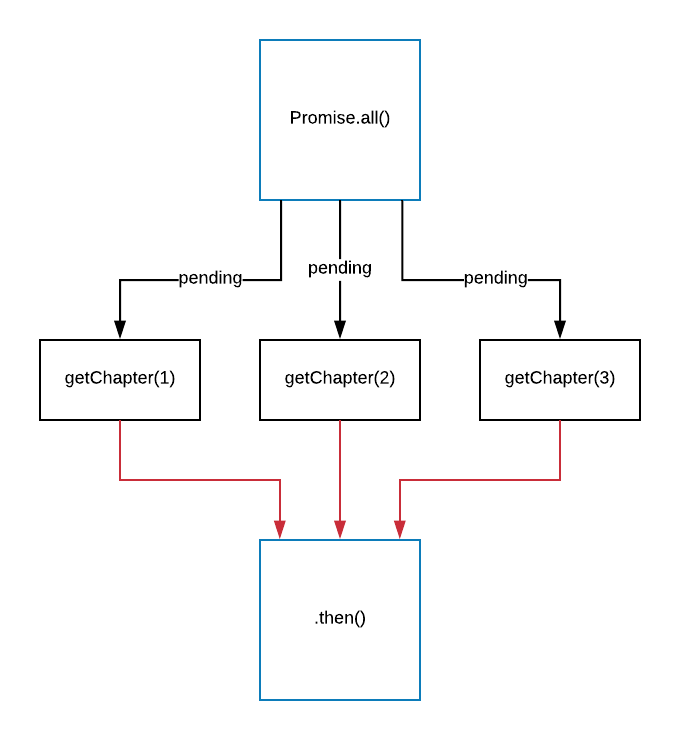
\includegraphics[width=7cm]{promise-all}
\caption{Die Nachrichten werden in der Reihenfolge ausgegeben, in der sie ins Array übergeben worden sind.}
\end{figure}

\noindent
Dagegen wird die nächste Methode verhältnismäßig seltener genutzt. Promise.race(iterable) gibt ein erfolgreiches oder fehlgeschlagenes Promise zurück, sobald eines der Promises in dem iterable erfolgreich war oder fehlgeschlagen ist, entsprechend mit dem Wert dieses Promises. Wenn das übergebene iterable leer ist, wird das Promise für immer im pending Status verharren.\cite{promise-race}

\begin{figure}[H]
\begin{lstlisting}[basicstyle=\small]
Promise.race(chapters).then((response) =>
    story.spawn(response)
).finally(() =>
    story.displayFinished()
);
\end{lstlisting}
\caption{Es wird schnellste ladende Kapitel angezeigt.}
\end{figure}

\subsection{Anti-Patterns und Best Practices}

Ob bei der Erstellung oder bei der Verarbeitung von Promises - Es gibt gewisse Ansätze nach denen man sich bei der Nutzung richten sollte. Ein negativ Beispiel für die Verarbeitung von Promises, wäre folgendes:

\begin{figure}[H]
\begin{lstlisting}[basicstyle=\small]
story.getChapter(1)
    .then((response1) => {
        story.spawn(response1);
        story.getChapter(2)
            .then((response2) => {
                story.spawn(response2);
                story.getChapter(3).then((response3) => {
                    story.spawn(response3);
                }).finally(() => {
                    story.spinnerElement.style.display = 'none';
                    story.displayFinished();
                });
            });
    });
\end{lstlisting}
\end{figure}

\noindent
Diese Methoden rufen ähnlich wie in Abbildung 13 drei Kapitel nacheinander auf. Obwohl sie im positiv Fall der API-Aufrufe die Kapitel sequentiell laden, wird hier komplett auf den Vorteil, den Promises gegenüber Callbacks bietet, verzichtet. Zudem ist die Ganze Kette davon abhängig, ob der erste Promise-Aufruf eintrifft. Hier wird keinerlei Möglichkeit gewährleistet ein Fehlschlag des ersten Aufrufs zu fangen ohne Code-Duplizierung. Solche ineinandergegliederte Promise-Verschachtelungen werden unter Entwicklern auch als \glqq{}Promise-Hell\grqq{} bezeichnet.
Mit dem ursprünglichen Beispiel ist es jedoch Möglich Fehler zwischen der Kette zu fangen:

\begin{figure}[H]
\begin{lstlisting}[basicstyle=\small]
story.getChapter(1)
    .then((response1) =>
        story.spawn(response1);
    )
    .catch((err) => ('Catched: ' + err))
    .then(() => story.getChapter(2)
        .then((response2) => 
            story.spawn(response2);
        ))
    ...
    \end{lstlisting}
\end{figure}

\noindent
Als Faustregel für Promises sollte beachtet werden, dass sie nur für einmalig auftretende asynchrone Events genutzt werden sollten. Der Verarbeitungsstatus eines Promise kann folgend sein:

\begin{itemize} 
\item Pending: Der Ausgang des Promises ist noch ungewiss.
\item Resolved: Die Aktion, die zum Promise verlief, ist eingetroffen.
\item Rejected: Die Aktion, die zum Promise verlief, schlug fehl.
\item Settled: Die Aktion ist entweder fehlgeschlagen oder eingetroffen - jedoch abgeschlossen.
\end{itemize}

\noindent
Beim erstellen einer Promise Instanz werden zwei Callback Funktionen als Argument angenommen. Resolve() wird mit der then() Methode verarbeitet und reject() mit der catch() Methode gefangen. Finally() kann unabhängig vom Eintreffen oder Fehlschlagen einer Operation genutzt werden. Der zurückgegebene Typ einer Promise Methode ist immer ein Promise-Objekt. Aufgrund dessen lassen sich Promises leicht verketten. Promises bieten mit Promise.all() und Promise.race() Hilfemethoden an, um mehrere Promises leichter zu verarbeiten.





\section{Reactive Programming}
In diesem Kapitel geht es rund um das Verstehen von \textbf{Reactive Programming}. Da es im Netz nur wenig Material zum Einstieg gibt bzw. das Thema nur oberflächlich angekratzt wird und die offizielle Dokumentation nur den Wenigsten zum Einleuchten bringt. Wird in dieser Arbeit die Herausforderung sein, die gesamte Architektur hinter den Observables zu erklären.
Sollte man von reactive Programming noch nichts gehört haben, dann wird die größte Schwierigkeit dabei sein in \glqq{}reactive\grqq{} zu denken.

\subsection{Funktionsweise}
Wenn es um reactive Programming geht, handelt es sich um das Entwickeln mit asynchronen Datenflüsse. Dabei können Datenflüsse aus verschiedensten Operationen entstehen wie z.B. Klick-Events, Variablen, Cache etc. Dabei kann man sich in diesem Datenfluss einhängen und entsprechend reagieren. Die Library \textbf{Reactive Extension for Javascript} (kurz: RxJS) bietet eine enorme Menge an Funktionen diese Datenflüsse zu bearbeiten/manipulieren. Diese Funktionen komplett abzudecken wird diese Arbeit unmöglich sein, jedoch wird nach dem behandeln dieser Sektion ein gewisses Grundverständnis für neue Operatoren entstehen und wie diese in Folge anzuwenden sind. Um einen Einblick zu gewähren, wird auf User-Events von einem Input-Feld eingegangen.

\noindent
Vor dem Ausführen des Beispiels muss folgend konfiguriert werden:

 \begin{center}
     Promises-vs.-Observables$\,\to\,$ webpack.config.js
 \end{center}

\begin{figure}[H]
\begin{lstlisting}
module.exports = {
    mode: 'development',
    entry: './src/modules/observables/introduction.ts',
    ...
}
\end{lstlisting}
\end{figure}

Da für es RxJS üblich ist für Operationsflüsse in Marbles-Diagramme darzustellen, werden diese in der Arbeit auch herangezogen.

\subsection{Unicast vs. Multicast}
\subsection{Hot Observables vs. Cold Observables}
\subsection{Operatoren}
\begin{enumerate} 
\item map, forEach, reduce (Operatoren ähnlich wie bei Arrays)
\item retry(), or replay() take(), take(), delay() distinctUnitlChanged() (Die das verhalten des Observers komplett verändern
\item mehrere Observable Operationen mit switchMap(), FlatMap(), concatMap()
\end{enumerate}

\section{Zusammenfassung}
\bibliography{references}

\end{document}
